\documentclass[12pt]{article}
\usepackage[utf8]{inputenc}
\usepackage{graphicx}
\usepackage[margin=1in]{geometry}
\usepackage{setspace}
\usepackage{float}
\setstretch{1.5}

\title{AXI VIP Tutorial 1}

\date{}

\begin{document}
%\maketitle
\section*{AXI VIP Tutorial 1}
\section*{Introduction}
The goal of this tutorial is to demonstrate how to use the Xilinx AXI Verification IP (VIP) to test and verify your custom AXI lite peripherals using the Xilinx Vivado Simulator. We will show you how to connect the VIP to your design and use it to write to and read from registers of the AXI GPIO IP. 

\section*{Step 1: Create a new project and block diagram}
\begin{enumerate}
	\item Create a new project for the \textbf{Nexys 4} board.
	\item Create a new block design and name it \textbf{design\_1}.
	\item Add and wire the \textbf{AXI Verification IP}, \textbf{AXI GPIO}, and \textbf{Constant} IPs to the diagram as shown in Figure \ref{fig:bd} below. Make sure that the port names match the figure.
		\begin{figure}[h]
		  \centering
		  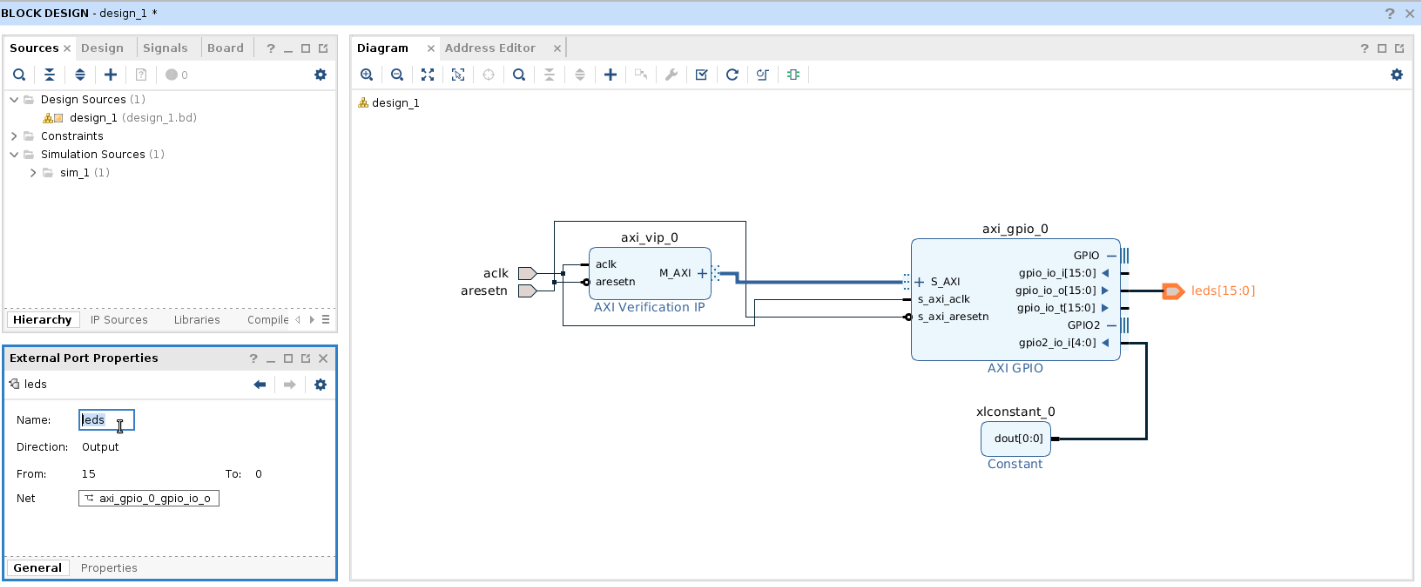
\includegraphics[width=\textwidth]{bd.png}
		  \caption{Block design.}
		  \label{fig:bd}
		\end{figure}
	\item Configure the \textbf{basic settings} tab of the \textbf{AXI VIP IP} as shown in the following figure. Leave the advance settings at their default values. This will set the VIP into AXI lite mode. 
		\begin{figure}[H]
		  \centering
		  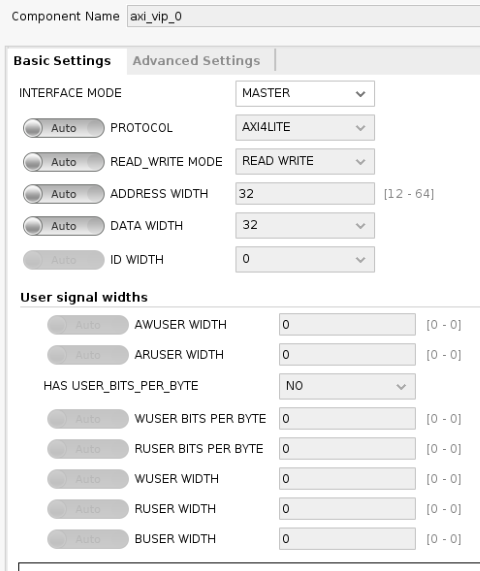
\includegraphics[scale=0.5]{axivipconfig.png}
		  \caption{AXI VIP configuration window.}
		  \label{fig:axivipconfig}
		\end{figure}
	\item Configure the \textbf{AXI GPIO IP} as shown in the following figure. We will be using the VIP to set the LEDs and read from the push buttons.
		\begin{figure}[H]
		  \centering
		  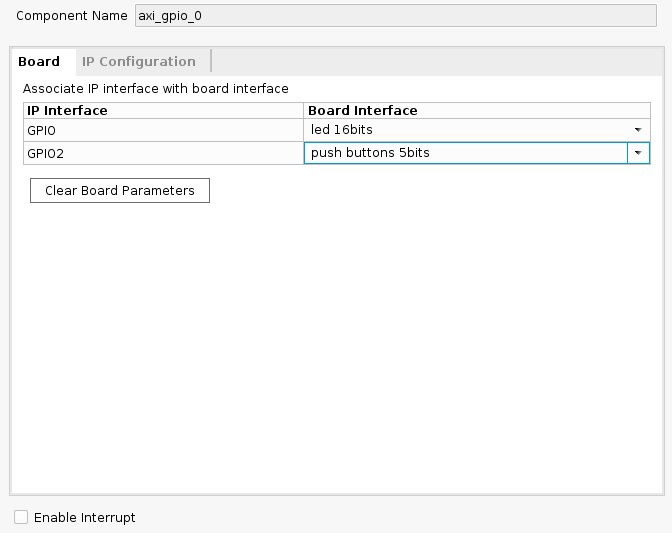
\includegraphics[scale=0.5]{axigpioconfig.png}
		  \caption{AXI GPIO configuration window.}
		  \label{fig:axigpioconfig}
		\end{figure}
	\item Configure the \textbf{Constant} IP as shown in the following figure. The constant value of 5 will simulate pushing buttons 0 and 2.
		\begin{figure}[H]
		  \centering
		  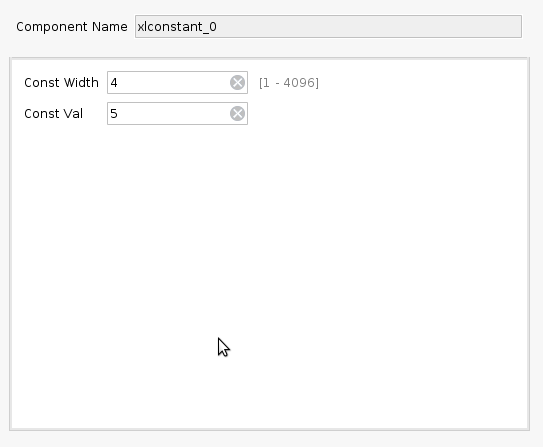
\includegraphics[scale=0.5]{axiconstantconfig.png}
		  \caption{Constant configuration window.}
		  \label{fig:axiconstantconfig}
		\end{figure}
	\item Go the \textbf{address editor} tab and set the offset address to \textbf{0x40000000}.
		\begin{figure}[H]
		  \centering
		  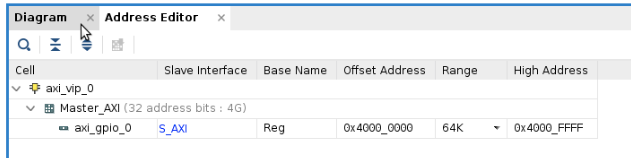
\includegraphics[scale=0.5]{addresseditor.png}
		  \caption{Address Editor}
		  \label{fig:addresseditor}
		\end{figure}
	\item Validate the block design, create the HDL wrapper, and generate the block design. 
		\begin{figure}[H]
		  \centering
		  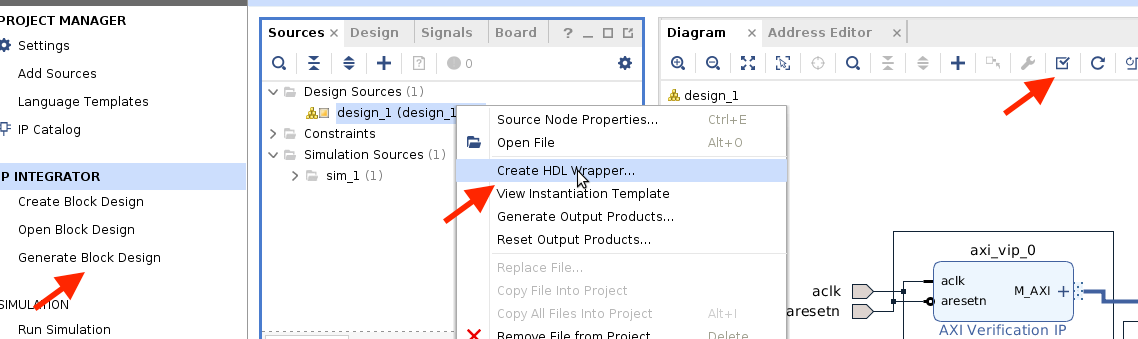
\includegraphics[scale=0.4]{validatebd.png}
		  \caption{Generating the block design files.}
		  \label{fig:validatebd.png}
		\end{figure}
\end{enumerate}
\section*{Step 2: Creating the testbench}
\begin{enumerate}
	\item Import \textbf{tb.sv} as a \textbf{simulation source}. 	
		\begin{figure}[H]
		  \centering
		  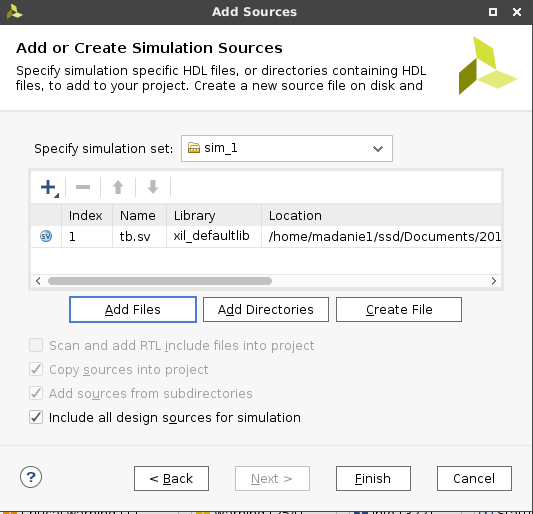
\includegraphics[scale=0.4]{addsimfiles.png}
		  \caption{Importing testbench files.}
		  \label{fig:addsimfilespng}
		\end{figure}
	\item Open the tb.sv file in Vivado text editor. Replace the \textbf{\textless vip\_component\_name\textgreater} in line 4 and 15 with the vip component name. Refer to Figure \ref{fig:findnames} to determine what the component name is for your design.
		\begin{figure}[H]
		  \centering
		  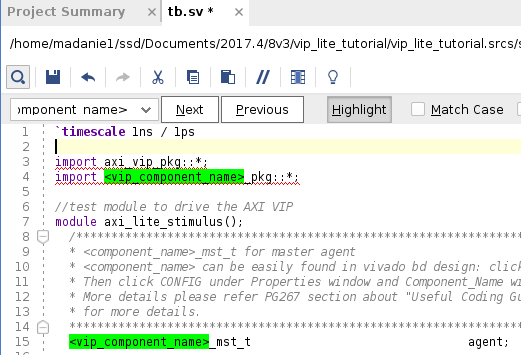
\includegraphics[scale=0.5]{componentname1.png}
		  \caption{Replace lines 4 and 15 with the appropriate component name for your VIP.}
		  \label{fig:componentname1}
		\end{figure}
		\begin{figure}[H]
		  \centering
		  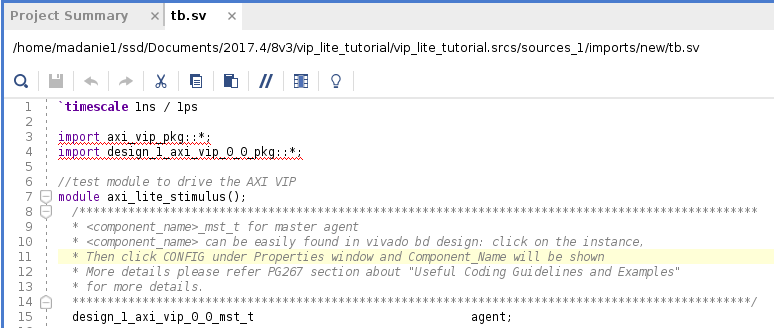
\includegraphics[scale=0.5]{componentname2.png}
		  \caption{Example of what lines 4 and 15 should look like.}
		  \label{fig:componentname2}
		\end{figure}
		\begin{figure}[H]
		  \centering
		  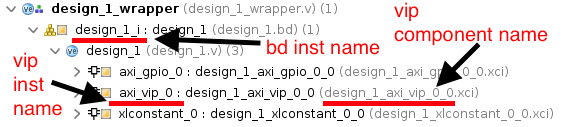
\includegraphics[scale=0.5]{filehierarchy2.png}
		  \caption{How to find the component and instance name.}
		  \label{fig:findnames}
		\end{figure}
		
	\item Go to line 60, and replace \textbf{\textless bd\_instance\_name\textgreater} and \textbf{\textless vip\_instance\_name\textgreater} with the bd instance name and vip instance name. Refer to Figure \ref{fig:findnames} to determine what the instance names are for your design.
		\begin{figure}[H]
		  \centering
		  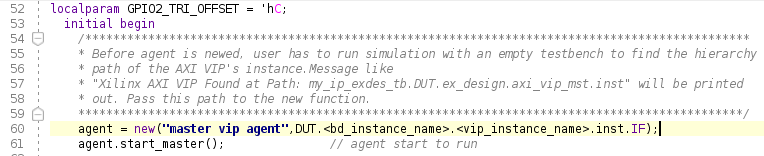
\includegraphics[scale=0.5]{instancename1.png}
		  \caption{Replace line 60 with the appropriate instance names for your BD and VIP.}
		  \label{fig:instancename1}
		\end{figure}
				\begin{figure}[H]
		  \centering
		  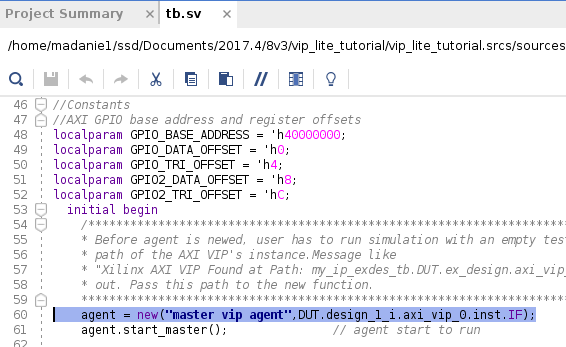
\includegraphics[scale=0.5]{instancename2.png}
		  \caption{Example of what line 60 should look like.}
		  \label{fig:instancename2}
		\end{figure}
	\item Set tb instance under Simulation Sources as the top instance if it isn't already. The simulation source hierarchy should look like the figure below. 
		\begin{figure}[H]
		  \centering
		  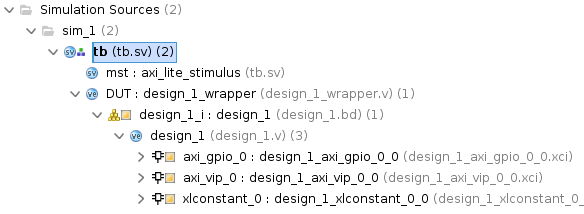
\includegraphics[scale=0.5]{filehierarchy.png}
		  \caption{Simulation source hierarchy.}
		  \label{fig:filehierarchy}
		\end{figure} 
\end{enumerate}
\section*{Step 3: Simulate the testbench}
\begin{enumerate}
	\item Before simulation, go to tb.sv and analyze line 66 to 75. This is where our test vectors are located. We will be writing to the output register of the GPIO bank that is connected to the LEDs. Then we'll set the push button GPIOs to be inputs and then wait for all writes to finish. We will then read the GPIO data register for the push buttons, and print the value of that register to the tcl console.
		\begin{figure}[H]
		  \centering
		  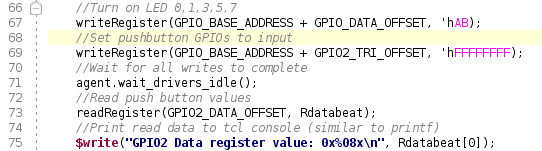
\includegraphics[scale=0.5]{tbanalysis.png}
		  \caption{TB test vectors.}
		  \label{fig:tbanalysis}
		\end{figure} 
	\item  Start the simulation by clicking "Run Simulation" on the navigation pane. Add the AXI bus signals to the simulation window and click relaunch simulation. Make sure that you select the VIP instance in the scope window.
		\begin{figure}[H]
		  \centering
		  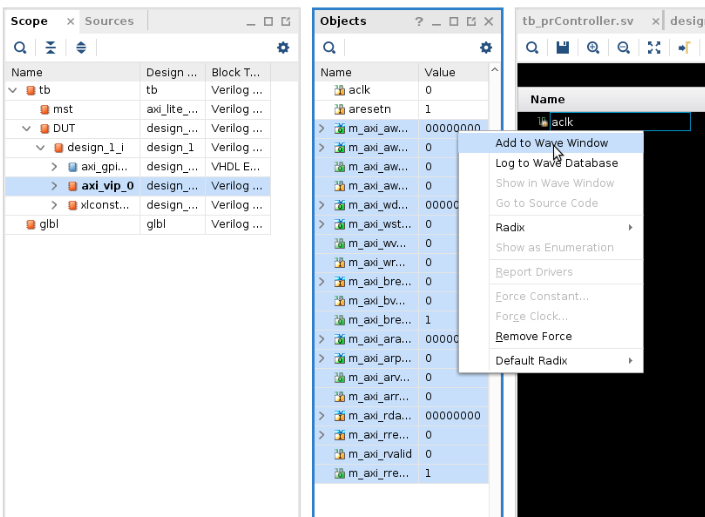
\includegraphics[scale=0.5]{addtbsignals.png}
		  \caption{Adding AXI signals to the simulation.}
		  \label{fig:addtbsignals}
		\end{figure} 
		\begin{figure}[H]
		  \centering
		  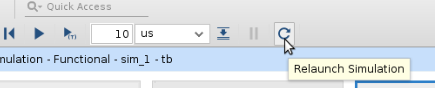
\includegraphics[scale=0.5]{relaunch.png}
		  \caption{Relaunching the simulation.}
		  \label{fig:relaunch}
		\end{figure} 
	\item Analyze the tb results...
		\begin{figure}[H]
		  \centering
		  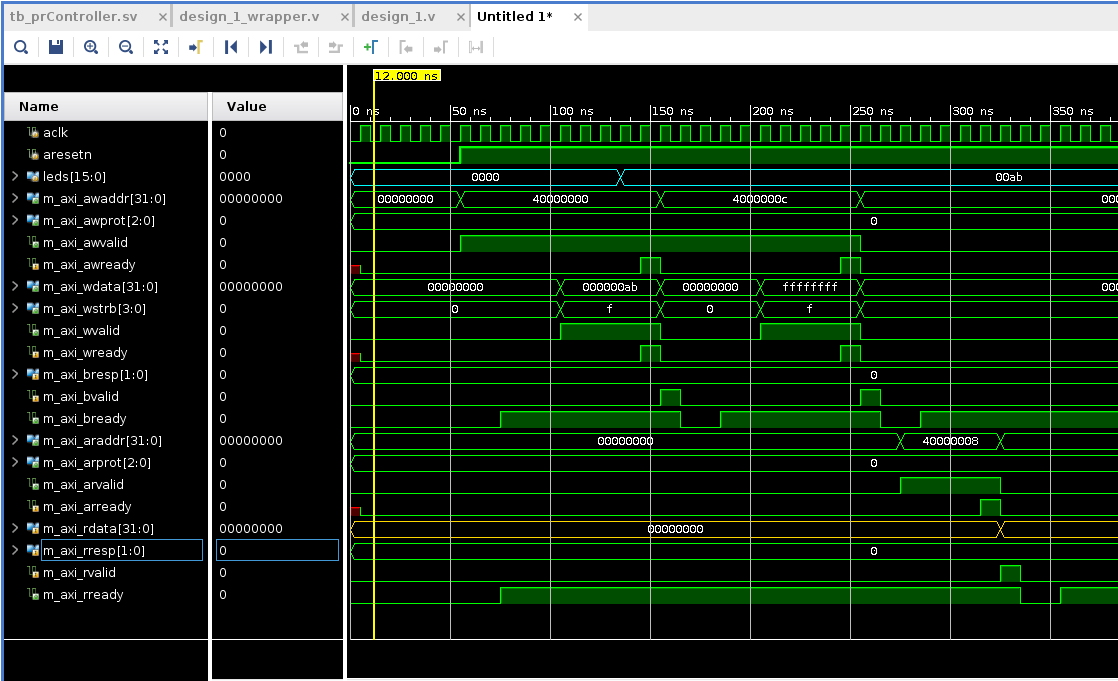
\includegraphics[scale=0.4]{simwaveform.png}
		  \caption{Simulation waveform.}
		  \label{fig:simwaveform.png}
		\end{figure} 
		\begin{figure}[H]
		  \centering
		  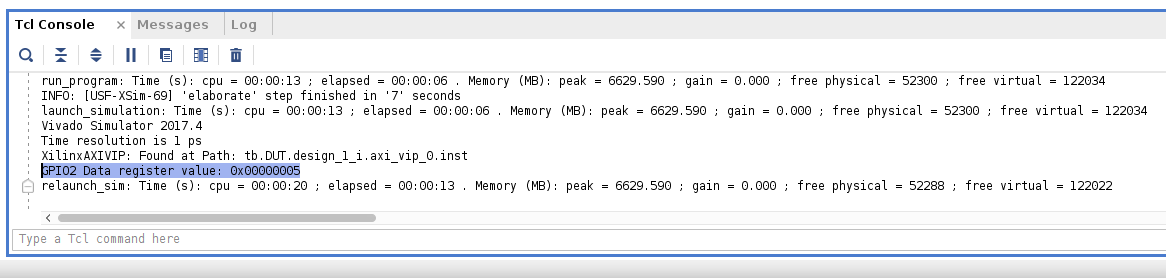
\includegraphics[scale=0.5]{simruntclconsole.png}
		  \caption{Tcl console print out of register.}
		  \label{fig:simruntclconsole}
		\end{figure} 
\end{enumerate}
\section*{Troubleshooting}
\begin{enumerate}
\item If the Vivado simulator bugs out and starts throwing errors that are not related to your source files, you can try to fix it by reseting your behaviour simulation.
		\begin{figure}[H]
		  \centering
		  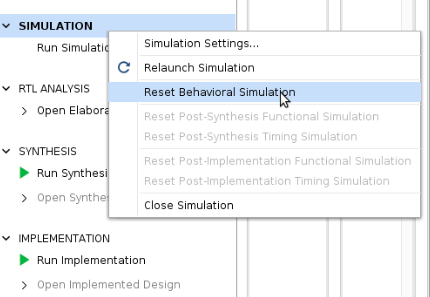
\includegraphics[scale=0.5]{troubleshoot1.png}
		  \caption{Resetting the simulation.}
		  \label{fig:roubleshoot1}
		\end{figure} 
\item If you want to create more advanced AXI testbenches with the Vivado AXI VIP refer to their example design.
		\begin{figure}[H]
		  \centering
		  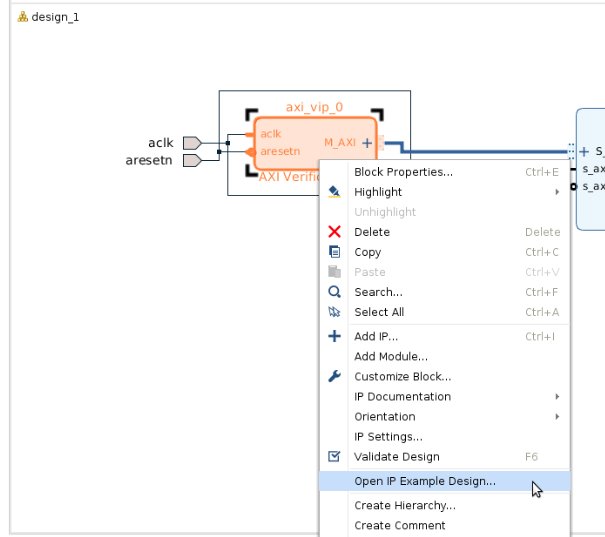
\includegraphics[scale=0.5]{exdesign.png}
		  \caption{Advanced example design for the AXI VIP.}
		  \label{fig:exdesign}
		\end{figure} 
\end{enumerate}
\end{document}
